\task{1.1}{Checking the mean-value formula}
We must prove that the average temperature on a small circle satisfies
\[
\frac{1}{2\pi}\int_0^{2\pi}u(x+\rho\cos\varphi,y+\rho\sin\varphi)\,\dd\varphi
=u(x,y)+\frac{\rho^2}{4}\lap u(x,y)+O(\rho^4).
\]
Here the circle radius is denoted by $\rho$, to distinguish it from the time-step parameter $r$ used later.

\textbf{Step 1: expand near the centre.}
Set $a=\rho\cos\varphi$, $b=\rho\sin\varphi$. With derivatives evaluated at $(x,y)$,
\begin{align*}
u(x+a,y+b)={}&u+a u_x+b u_y
+\frac12\bigl(a^2u_{xx}+2ab u_{xy}+b^2u_{yy}\bigr)\\
&+\frac16\bigl(a^3u_{xxx}+3a^2b u_{xxy}+3ab^2u_{xyy}+b^3u_{yyy}\bigr)
+O(\rho^4).
\end{align*}
The problem asks us to compute the second-order terms. The cubic terms are displayed as well
to justify the stated $O(\rho^4)$ remainder: a second-order expansion alone would give only
an $O(\rho^3)$ pointwise remainder.

\textbf{Step 2: average the constant and linear terms.}
The average of $u$ is $u$. Also,
\[
\int_0^{2\pi}\cos\varphi\,\dd\varphi
=\int_0^{2\pi}\sin\varphi\,\dd\varphi=0,
\]
so the linear terms contribute nothing.

\textbf{Step 3: average the quadratic terms.}
Using
\[
\int_0^{2\pi}\cos^2\varphi\,\dd\varphi
=\int_0^{2\pi}\sin^2\varphi\,\dd\varphi=\pi,
\qquad \int_0^{2\pi}\cos\varphi\sin\varphi\,\dd\varphi=0,
\]
the quadratic contribution is
\[
\frac{1}{2\pi}\frac{\rho^2}{2}
\bigl(\pi u_{xx}+0+\pi u_{yy}\bigr)
=\frac{\rho^2}{4}(u_{xx}+u_{yy}).
\]

\textbf{Step 4: account for the remainder.}
Each cubic monomial changes sign under $\varphi\mapsto\varphi+\pi$, so its integral
over a full circle is zero. The remaining term is uniformly $O(\rho^4)$ when $u$ has bounded
fourth derivatives near the circle. Its average is also $O(\rho^4)$. Therefore
\[
\boxed{\ \text{circle average}=u+\frac{\rho^2}{4}\lap u+O(\rho^4).\ }
\]
Thus a positive Laplacian means that the nearby surroundings are warmer on average than the
centre. In the heat equation, this makes the centre warm up.

\task{1.2}{Dimensional analysis}
\partsol{a}
Write $[L]$ for length units and $[\mathrm{time}]$ for time units. Thermal diffusivity has units
$[\alpha]=[L]^2/[\mathrm{time}]$. Consequently,
\[
\left[\frac{\alpha t}{L^2}\right]
=\frac{([L]^2/[\mathrm{time}])[\mathrm{time}]}{[L]^2}=1.
\]
Therefore $\alpha t/L^2$ is dimensionless.

\partsol{b}
Seek a time scale of the form $\alpha^a L^b$. Its units are
\[
[\alpha^aL^b]=[L]^{2a+b}[\mathrm{time}]^{-a}.
\]
Matching the units of time requires $-a=1$ and $2a+b=0$.
Hence $a=-1$, $b=2$, and the only such monomial, up to a dimensionless constant, is
\[
\boxed{\tau=\frac{L^2}{\alpha}.}
\]
If $L$ and $\alpha$ are the only dimensional parameters, a spreading time must have the form
$t_{\mathrm{spread}}=C L^2/\alpha$. The dimensionless constant $C$ depends on the shape,
boundary conditions, and what is meant by ``spread''; dimensional analysis does not determine it.

For $L=10\,\mathrm{cm}=0.10\,\mathrm{m}$, using the diffusivities supplied in the notes,
\begin{align*}
\tau_{\mathrm{copper}}&=\frac{0.10^2}{1.1\times10^{-4}}
\simeq90.9\,\mathrm{s}\simeq1.52\,\mathrm{min},\\
\tau_{\mathrm{steel}}&=\frac{0.10^2}{1.3\times10^{-5}}
\simeq769.2\,\mathrm{s}\simeq12.8\,\mathrm{min}.
\end{align*}
Steel's characteristic time is approximately $8.46$ times larger. This agrees with the
expectation that heat spreads faster through copper. These are diffusion scales, not exact
times at which the plate reaches equilibrium.

\partsol{c}
Define
\[
\hat x=x/L,\qquad \hat y=y/L,\qquad \hat t=\alpha t/L^2,
\]
and let $\hat u(\hat x,\hat y,\hat t)=u(L\hat x,L\hat y,L^2\hat t/\alpha)$.
By the chain rule,
\[
u_t=\frac{\alpha}{L^2}\hat u_{\hat t},\qquad
u_{xx}=\frac{1}{L^2}\hat u_{\hat x\hat x},\qquad
u_{yy}=\frac{1}{L^2}\hat u_{\hat y\hat y}.
\]
Substitution in $u_t=\alpha(u_{xx}+u_{yy})$ and cancellation of $\alpha/L^2$ give
\[
\boxed{\hat u_{\hat t}=\hat u_{\hat x\hat x}+\hat u_{\hat y\hat y}.}
\]
Neither $\alpha$ nor $L$ appears in this equation. A solver for unit diffusivity on a unit square
therefore describes any geometrically similar square plate after rescaling coordinates and time:
$x=L\hat x$, $y=L\hat y$, $t=(L^2/\alpha)\hat t$. Initial and boundary data must be transformed
too. A rectangle with unequal sides retains its aspect ratio; scaling does not change its shape.

\task{1.3}{Fourier modes}
Let
\[
\beta_x=\frac{m\pi}{L_x},\qquad \beta_y=\frac{n\pi}{L_y},\qquad
\lambda=\alpha(\beta_x^2+\beta_y^2),
\]
where $m,n$ are positive integers. The proposed function is
\[
u_{mn}(x,y,t)=\sin(\beta_xx)\sin(\beta_yy)e^{-\lambda t}.
\]
\textbf{Step 1: differentiate in time.}
The sine factors are independent of time, so
\[
(u_{mn})_t=-\lambda u_{mn}.
\]
\textbf{Step 2: differentiate twice in each spatial direction.}
Since $(\sin(\beta x))''=-\beta^2\sin(\beta x)$,
\[
(u_{mn})_{xx}=-\beta_x^2u_{mn},\qquad
(u_{mn})_{yy}=-\beta_y^2u_{mn}.
\]
It follows that
\[
\alpha\lap u_{mn}
=-\alpha(\beta_x^2+\beta_y^2)u_{mn}
=-\lambda u_{mn}=(u_{mn})_t.
\]
\textbf{Step 3: check every boundary.}
At $x=0$, the first sine is zero; at $x=L_x$, it is $\sin(m\pi)=0$.
Similarly the second sine vanishes at $y=0,L_y$. Thus all four Dirichlet conditions hold.

\textbf{Step 4: evaluate the initial data.}
At $t=0$ the exponential is one, so
\[
\boxed{u_0(x,y)=\sin\!\left(\frac{m\pi x}{L_x}\right)
\sin\!\left(\frac{n\pi y}{L_y}\right).}
\]
Each mode retains its spatial shape while its amplitude decays exponentially. The decay rate
increases quadratically with mode number, explaining why fine spatial oscillations disappear
more rapidly than broad temperature variations.

\task{2.1}{Taylor expansions}
All derivatives in this task are evaluated at $x$.
\partsol{a}
Taylor's formula gives
\[
\boxed{f(x+h)=f+hf'+\frac{h^2}{2}f''+\frac{h^3}{6}f'''
+\frac{h^4}{24}f^{(4)}+O(h^5).}
\]
\partsol{b}
Replace $h$ by $-h$:
\[
\boxed{f(x-h)=f-hf'+\frac{h^2}{2}f''-\frac{h^3}{6}f'''
+\frac{h^4}{24}f^{(4)}+O(h^5).}
\]
Terms containing odd powers of $h$ change sign, since $(-h)^k=-h^k$ for odd $k$.
Even powers do not change sign. This distinction makes it possible to cancel selected Taylor
terms by adding or subtracting symmetric samples.
\partsol{c}
Replace $h$ by $2h$:
\begin{align*}
f(x+2h)&=f+2hf'+\frac{(2h)^2}{2}f''+\frac{(2h)^3}{6}f'''
+\frac{(2h)^4}{24}f^{(4)}+O((2h)^5)\\
&=\boxed{f+2hf'+2h^2f''+\frac43h^3f'''+\frac23h^4f^{(4)}+O(h^5).}
\end{align*}
The factor $2^5$ in the remainder is constant, so it is absorbed in the $O(h^5)$ notation.

\task{3.1}{The backward difference}
The backward approximation is
\[
D_-f(x)=\frac{f(x)-f(x-h)}{h}.
\]
Insert the expansion from Task 2.1(b):
\begin{align*}
f(x)-f(x-h)
&=hf'-\frac{h^2}{2}f''+\frac{h^3}{6}f'''-\frac{h^4}{24}f^{(4)}+O(h^5),\\
D_-f(x)&=f'-\frac{h}{2}f''+\frac{h^2}{6}f'''-\frac{h^3}{24}f^{(4)}+O(h^4).
\end{align*}
Thus, defining truncation error as approximation minus exact derivative,
\[
\boxed{D_-f(x)-f'(x)=-\frac{h}{2}f''(x)+O(h^2)=O(h).}
\]
The method is first-order accurate. For a generic function the leading error is proportional to
$h$, so halving $h$ approximately halves the error. Its leading sign is opposite to that of
the forward difference. A particular function or point can have $f''(x)=0$ and a smaller error;
this does not change the general order of the formula.

\task{3.2}{A finite difference for the second derivative}
\partsol{a}
Add the symmetric Taylor expansions instead of subtracting them:
\[
f(x+h)+f(x-h)=2f(x)+h^2f''(x)+\frac{h^4}{12}f^{(4)}(x)+O(h^6).
\]
Here the stronger $O(h^6)$ form follows by expanding through degree five and cancelling odd
terms, assuming sufficient smoothness. Subtract $2f(x)$ and divide by $h^2$:
\[
\boxed{D_2f(x)=\frac{f(x-h)-2f(x)+f(x+h)}{h^2}\approx f''(x).}
\]
The same coefficients follow systematically from
\[
D_2f=\frac{af(x-h)+bf(x)+cf(x+h)}{h^2}.
\]
After expansion, cancelling the constant and first derivative and matching $f''$ gives
\[
a+b+c=0,\qquad -a+c=0,\qquad \frac{a+c}{2}=1.
\]
Hence $a=c=1$ and $b=-2$.

\partsol{b}
The expansion above gives
\[
\boxed{D_2f(x)-f''(x)=\frac{h^2}{12}f^{(4)}(x)+O(h^4).}
\]
The leading truncation error is $h^2 f^{(4)}(x)/12$, so the method is second-order accurate.
If only the expansions through degree four with $O(h^5)$ remainders are used, one obtains
the same leading term and an $O(h^3)$ remainder, already sufficient to establish order two.

\partsol{c}
For $f(x)=\sin x$,
\[
f''(1)=-\sin1\simeq-0.8414709848078965,\qquad f^{(4)}(1)=\sin1.
\]
The experiment evaluates the three-point quotient directly in double precision.
\begin{center}
\begin{tabular}{rrrr}
\toprule
$h$ & $D_2f(1)$ & $|D_2f(1)-f''(1)|$ & Previous error / error\\
\midrule
\tableinput{tables/task_3_2.tex}
\bottomrule
\end{tabular}
\end{center}
The ratios approach $4=2^2$, confirming second-order accuracy. The error is positive before
taking the absolute value, as predicted by $h^2\sin1/12$: the approximation is slightly less
negative than the exact second derivative.

\task{3.3}{Sanity checks on the second derivative}
\partsol{a}
For a constant function $f(x)=1$,
\[
D_2f(x)=\frac{1-2+1}{h^2}=0.
\]
For $f(x)=x$,
\[
D_2f(x)=\frac{(x-h)-2x+(x+h)}{h^2}=0.
\]
For $f(x)=x^2$,
\begin{align*}
D_2f(x)&=\frac{(x-h)^2-2x^2+(x+h)^2}{h^2}\\
&=\frac{(x^2-2xh+h^2)-2x^2+(x^2+2xh+h^2)}{h^2}=2.
\end{align*}
These are the exact derivatives: constants and straight lines have no curvature, and $x^2$
has curvature $2$. For a consistent fixed-coefficient three-point formula divided by $h^2$,
the corresponding Taylor moment conditions must cancel constants and linear terms and normalize
the quadratic term. A failure of these tests reveals an incorrect coefficient or scaling.

\partsol{b}
The coefficient sum is
\[
\frac{1-2+1}{h^2}=0.
\]
Consequently adding the same constant temperature to all three samples leaves the computed
second derivative unchanged. This expresses the fact that curvature depends on relative values,
not on the choice of temperature origin.

\partsol{c}
Define the neighbour average by
\[
\bar f=\frac{f(x-h)+f(x+h)}{2}.
\]
Then
\[
\boxed{D_2f(x)=\frac{2}{h^2}\bigl(\bar f-f(x)\bigr).}
\]
The second difference is positive if the centre is below its neighbours' average, negative if
it is above that average, and zero if they balance. In heat diffusion, this determines whether
the centre warms or cools.

\task{3.4}{The discrete Laplacian}
\partsol{a}
Hold $y=y_j$ fixed and apply the second difference in $x$:
\[
\boxed{u_{xx}(x_i,y_j)\approx
\frac{u_{i+1,j}-2u_{i,j}+u_{i-1,j}}{\Delta x^2}.}
\]
\partsol{b}
Hold $x=x_i$ fixed and apply it in $y$:
\[
\boxed{u_{yy}(x_i,y_j)\approx
\frac{u_{i,j+1}-2u_{i,j}+u_{i,j-1}}{\Delta y^2}.}
\]
\partsol{c}
Adding gives the discrete Laplacian
\[
\boxed{\lap_hu_{i,j}=
\frac{u_{i+1,j}-2u_{i,j}+u_{i-1,j}}{\Delta x^2}
+\frac{u_{i,j+1}-2u_{i,j}+u_{i,j-1}}{\Delta y^2}.}
\]
For samples of a smooth exact function, its error is
\[
\lap_hu-\lap u
=\frac{\Delta x^2}{12}u_{xxxx}+\frac{\Delta y^2}{12}u_{yyyy}
+O(\Delta x^4+\Delta y^4).
\]
Thus the spatial approximation is $O(\Delta x^2+\Delta y^2)$.
No mixed derivative is needed because the Laplacian itself is the sum of the two pure second derivatives.

\partsol{d}
If $\Delta x=\Delta y=h$,
\[
\boxed{\lap_hu_{i,j}=
\frac{u_{i-1,j}+u_{i+1,j}+u_{i,j-1}+u_{i,j+1}-4u_{i,j}}{h^2}.}
\]
\partsol{e}
The following array marks the five nodes and their weights. Empty positions are unused;
the common factor is $1/h^2$.
\[
\frac{1}{h^2}
\begin{array}{c|ccc}
 & i-1&i&i+1\\\hline
j+1&&1&\\
j&1&-4&1\\
j-1&&1&
\end{array}
\qquad
\begin{array}{c}
\text{north: }(i,j+1)\\
\text{west, centre, east: }(i-1,j),(i,j),(i+1,j)\\
\text{south: }(i,j-1)
\end{array}
\]
For unequal spacings the west/east weights are $1/\Delta x^2$, the north/south weights
are $1/\Delta y^2$, and the centre weight is $-2/\Delta x^2-2/\Delta y^2$.
Diagonal nodes such as $(i+1,j+1)$ do not belong to this stencil.

\partsol{f}
Let $\bar u_4$ be the arithmetic mean of the four neighbouring samples. Then
\[
\lap_hu_{i,j}=\frac{4}{h^2}(\bar u_4-u_{i,j}),
\qquad
\bar u_4=u_{i,j}+\frac{h^2}{4}\lap u+O(h^4).
\]
Task 1.1 gives the same leading expression for the circular average at radius $h$.
Both measure the difference between the centre and its surroundings. The averages need not
coincide exactly: the four-point average samples only the coordinate directions, and their
fourth-order terms can differ.

\task{3.5}{Where round-off takes over}
We repeat the direct quotient in Task 3.2 at $x=1$ for $h=10^{-1},\ldots,10^{-10}$.
The computed values are:
\begin{center}
\begin{tabular}{rrr}
\toprule
$h$ & Computed $D_2\sin(1)$ & Absolute error\\
\midrule
\tableinput{tables/task_3_5.tex}
\bottomrule
\end{tabular}
\end{center}
\begin{figure}[H]
\centering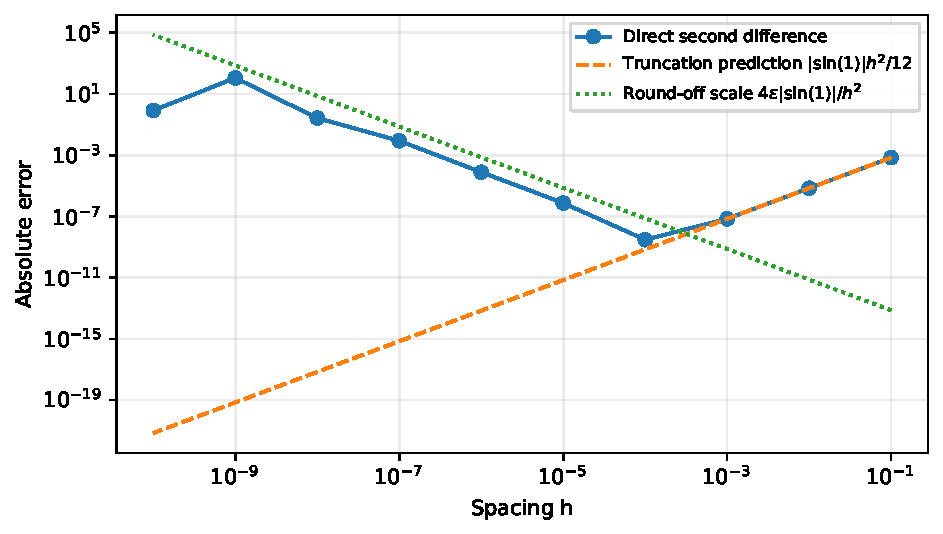
\includegraphics[width=.88\linewidth]{task_3_5_roundoff.pdf}
\caption{Direct second-difference error in double precision. The round-off curve is a scale
estimate, not a pointwise bound; cancellation makes the measured error irregular.}
\end{figure}
\textbf{Observed transition.} In this run the smallest error among the sampled spacings occurs
at $h=10^{-4}$. Reducing $h$ to $10^{-5}$ increases the error sharply. Thus the transition
is near $10^{-4}$, with the precise location depending on floating-point rounding.

\textbf{Why this happens.} The truncation error is approximately
$C h^2$, where $C=|\sin1|/12$. Each sampled function value contains rounding error.
The coefficients $1,-2,1$ combine errors of scale $\epsilon |f|$, and division by $h^2$
amplifies them. A useful model is
\[
E(h)\approx C h^2+\frac{D\epsilon}{h^2},\qquad \epsilon\simeq2.22\times10^{-16},
\]
where $D$ is a function-dependent constant of order one. Differentiating this model gives
\[
2Ch-2D\epsilon h^{-3}=0
\quad\Longrightarrow\quad
h_{\mathrm{opt}}^4=\frac{D\epsilon}{C}.
\]
Therefore $h_{\mathrm{opt}}$ has scale $\epsilon^{1/4}$, roughly $10^{-4}$.
The $\sqrt\epsilon$ scale discussed for the forward \emph{first} derivative does not apply here:
the second derivative has both a different truncation error and a division by $h^2$.

For extremely small $h$, nearly equal sine values are subtracted, and the numerator may round
to zero or to a small multiple of machine precision. Dividing that unreliable residual by $h^2$
can produce a very large error. Smaller spacing is therefore useful only until round-off
overtakes truncation error. The exact last digits of this table can vary between math libraries.
